\documentclass{article}
\usepackage[utf8]{inputenc}
\usepackage[T1]{fontenc}
\usepackage{graphicx}
\usepackage{amsmath, amssymb}
\usepackage{xcolor}
\usepackage{tikz}
\usepackage{enumitem}
\usepackage{lipsum}
\usetikzlibrary{fit}
\usepackage{hyperref} 
\usepackage{subfig}
\usepackage{polynom}
\usepackage{pgfplots}
\usepackage{soul}
\usepackage{framed}
\usepackage[most]{tcolorbox}
% Define colors
\definecolor{lessoncolor}{RGB}{74, 144, 226}
\definecolor{examplecolor}{RGB}{92, 184, 92}
\definecolor{notecolor}{RGB}{255, 179, 102}



% Define a command for colorful sections
\newcommand{\colorsection}[1]{\section*{\textcolor{lessoncolor}{#1}}}
\newcommand{\xdownarrow}[1]{%
  {\left\downarrow\vbox to #1{}\right.\kern-\nulldelimiterspace}
}

\definecolor{antiquefuchsia}{rgb}{0.57, 0.36, 0.51}

% Set up TikZ for graphing
\usetikzlibrary{positioning, arrows.meta, shapes.geometric}
\usetikzlibrary{decorations.pathreplacing}

% Document
\begin{document}

\begin{titlepage}
    \centering
    \vspace*{2cm}
    {\LARGE \textcolor{lessoncolor}{Advanced Functions}}\par
    \vspace{1cm}
    {\large Kensukeken}\par
    \vspace{2cm}
    {\large April 2nd, 2024}\par
    \vspace{3cm}
\end{titlepage}
\tableofcontents
\newpage
\section{Unit 3}
\subsection{Reciprocal of a Linear Function}
$$y=mx+b$$
Reciprocal function\\\\
\begin{minipage}{0.5\textwidth}
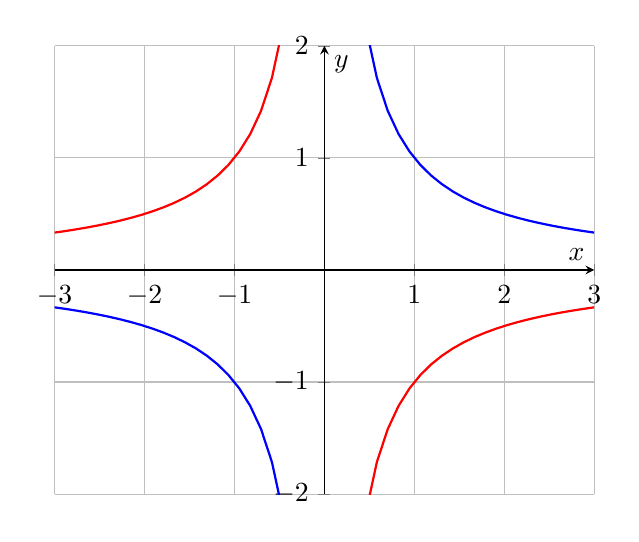
\begin{tikzpicture}
    \begin{axis}[
        grid=both,
        axis lines=middle,
        xmin=-3, xmax=3,
        ymin=-2, ymax=2,
        xlabel={$x$},
        ylabel={$y$},
        ]
        \addplot[blue, thick, domain=-3:-0.1] {1/x};
        \addplot[blue, thick, domain=0.1:3] {1/x};
        \addplot[red, thick, domain=3:0.1]{-1/x};
        \addplot[red, thick, domain=-0.1:-3]{-1/x};
    \end{axis}
\end{tikzpicture}
\end{minipage}
\hspace{1cm}
\begin{minipage}{0.4\textwidth}
\centering
\begin{tabular}{|c|c|c|c|}

$x$ & $\frac{1}{x}$ & $-\frac{1}{x}$ \\ 
\hline
-3 & -0.33 & -0.33 \\
\hline
-2 & -0.5 & -0.5 \\
\hline
-1 & -1 & -1 \\
\hline
1 & 1 & -1 \\
\hline 
2 & 0.5 & -0.5 \\
\hline
3 & 0.33 & -0.33 \\

\end{tabular}
\end{minipage}
\noindent
The reciprocal function $f(x) = \frac{1}{x}$ has \hl{two hyperbolas} in the 1st and 3rd quadrants. As $x$ approaches 0 from either side, $f(x)$ approaches $\pm\infty$. 
\subsubsection{End Behaviour}
\begin{align*}
    x \to -\infty, y=0^-\\
    x \to +\infty, y\to 0^+\\
    x \to 0^-, y \to-\infty\\
    x\to 0^+, y\to+\infty\\
    x\in (-\infty,0) \quad y \downarrow \\
    x > 0 \quad  y \downarrow \\
    x \in (0, +\infty) \quad y \downarrow 
\end{align*}

\subsubsection{Domain and Range}
\begin{equation*}
    D: \{x \in \mathbb{R} | x \neq 0\}, 
    R: \{y \in \mathbb{R} | y \neq 0\} 
\end{equation*}
\subsubsection*{Example 1:}
Solve for $f(x)=\frac{1}{-3x+5}$
\begin{enumerate}
\item[a)] State the domain and range.
\item[b)] Describe the behaviour of the function near the vertical asymptote.
\item[c)] Describe the end behaviour.
\item[d)] Sketch a graph of the function.
\end{enumerate}
\subsubsection*{Solution}
\begin{enumerate}
    \item[a)] \textbf{Domain \& Range}:
    The function \( f(x) = \frac{1}{-3x + 5} \) will be undefined when the denominator equals zero because division by zero is undefined. So, we solve for \( x \):
    \[ -3x + 5 = 0 \]
    \[ -3x = -5 \]
    \[ x = \frac{5}{3} \]
    So, the domain of the function is all real numbers except \( x = \frac{5}{3} \). 
    The range is $R: \{y \in \mathbb{R} | y \neq 0\}$
    
    \item[b)] \textbf{Behaviour near the vertical asymptote}:
    The vertical asymptote occurs when the denominator approaches zero, which in this case is \( x = \frac{5}{3} \). Near this point, the function behaves similarly to \( \frac{1}{x} \), approaching positive or negative infinity depending on whether \( x \) approaches \( \frac{5}{3} \) from the left or the right, respectively.
    
    \item[c)] \textbf{End behaviour}:
    As \( x \) approaches positive or negative infinity, \( f(x) \) approaches zero. This is because the term \( -3x \) dominates the function as \( x \) becomes very large in magnitude, making the entire fraction approach zero.
    
    \item[d)] \textbf{Sketch of the graph}:
    The graph will be a hyperbola with a vertical asymptote at \( x = \frac{5}{3} \) and approaching the x-axis as \( x \) approaches positive or negative infinity.
    \begin{figure}[ht]
    \centering
    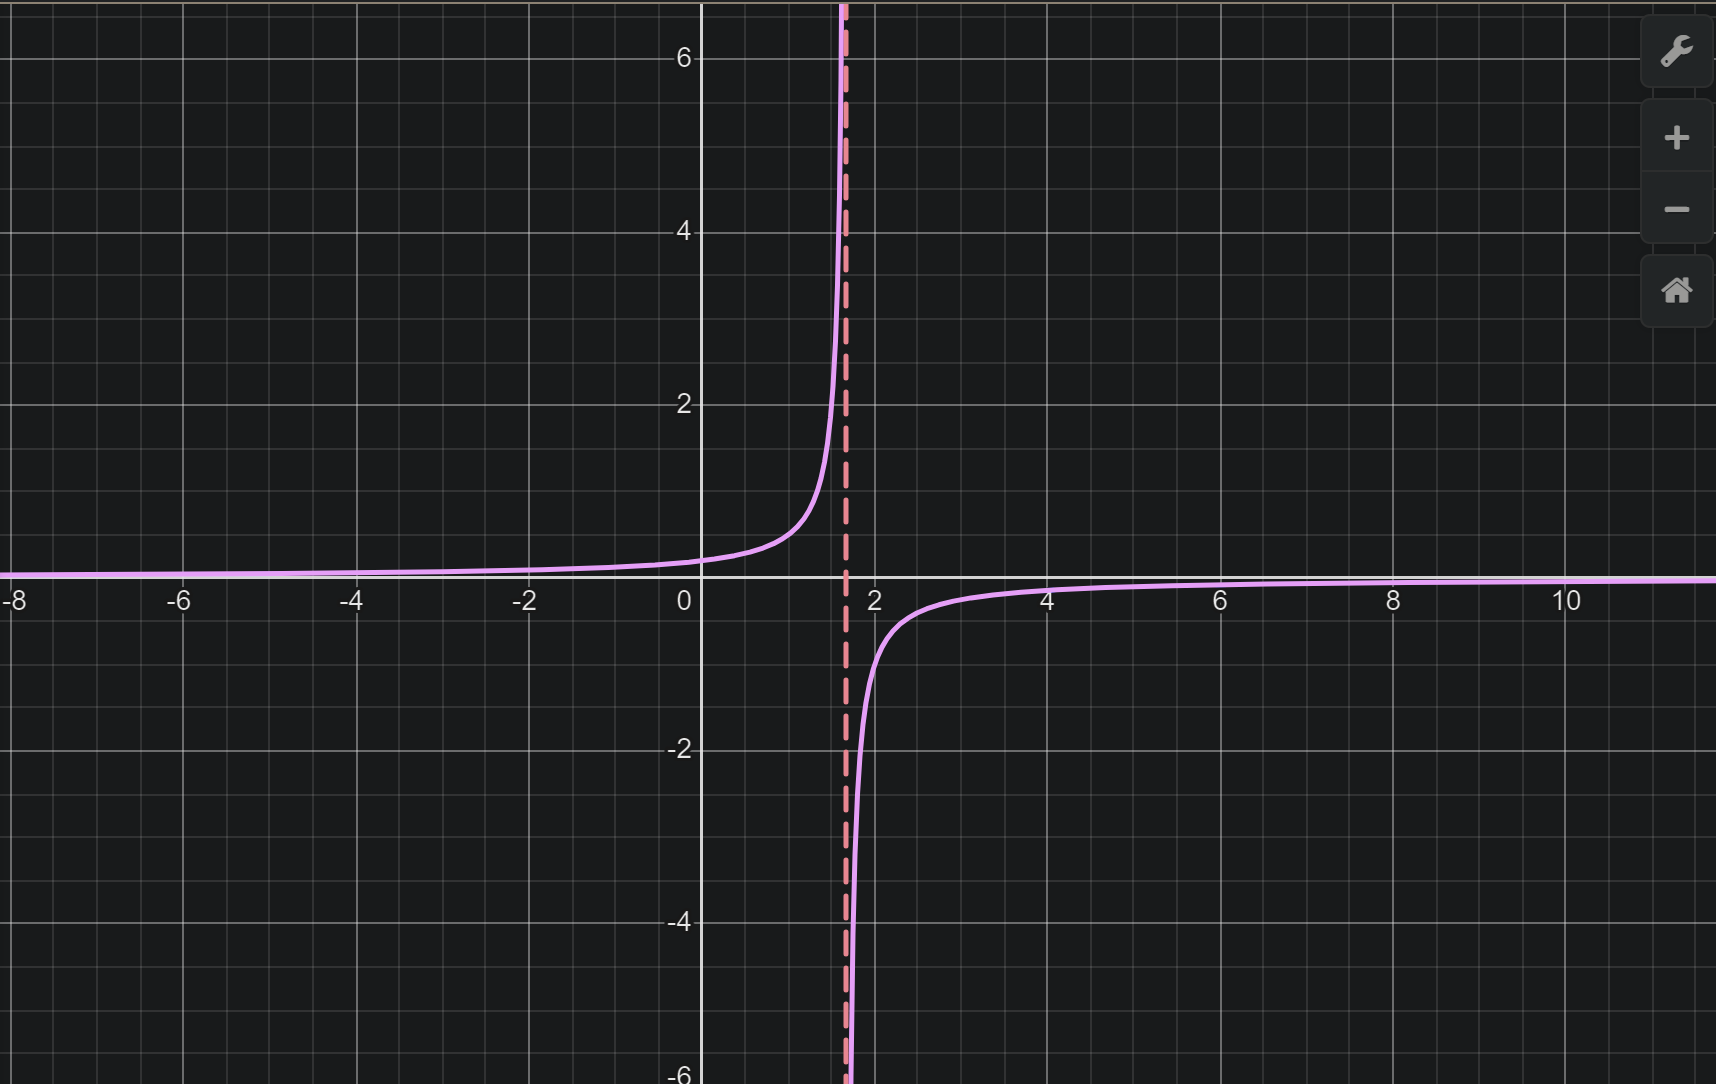
\includegraphics[width=0.9\textwidth]{imgs/graph(1_3x+5).png}
    \end{figure}
    \\
    $x\to \frac{5}{3}^-, y\to \infty$, $x\in (-\infty,\frac{5}{3})$ increase\\
    $x \to \frac{5}{3}^+, y\to -\infty$, $x\in(\frac{5}{3}, +\infty)$ increase
\end{enumerate}

\subsubsection*{Example 2:}
Solve for $f(x)=\frac{1}{(x+1)(x-3)}$
\begin{enumerate}
\item[a)] State the domain and range.
\item[b)] Describe the behaviour of the function near the vertical asymptote.
\item[c)] Describe the end behaviour.
\item[d)] Sketch a graph of the function.
\end{enumerate}
\subsubsection*{Solution:}

\begin{enumerate}
    \item[a)] \text{Domain and Range:}
    The function \( f(x) = \frac{1}{(x+1)(x-3)} \) is undefined at \( x = -1 \) and \( x = 3 \).     So, the domain of the function is all real numbers except \( x = -1 \) and \( x = 3 \). The range is all real numbers except when \( f(x) \) equals zero.
    
    \item[b)] \text{Behaviour near the vertical asymptotes}:
    Near \( x = -1 \) and \( x = 3 \), the function behaves like \( \frac{1}{x} \), approaching infinity as \( x \) approaches these points.
    
    \item[c)] \text{End behaviour }
    As \( x \) tends to positive or negative infinity, \( f(x) \) approaches zero due to the dominance of \( (x+1) \) and \( (x-3) \) in the denominator.
    \item[d)] \text{Sketch of the graph:}
    \begin{figure}[ht]
    \centering
    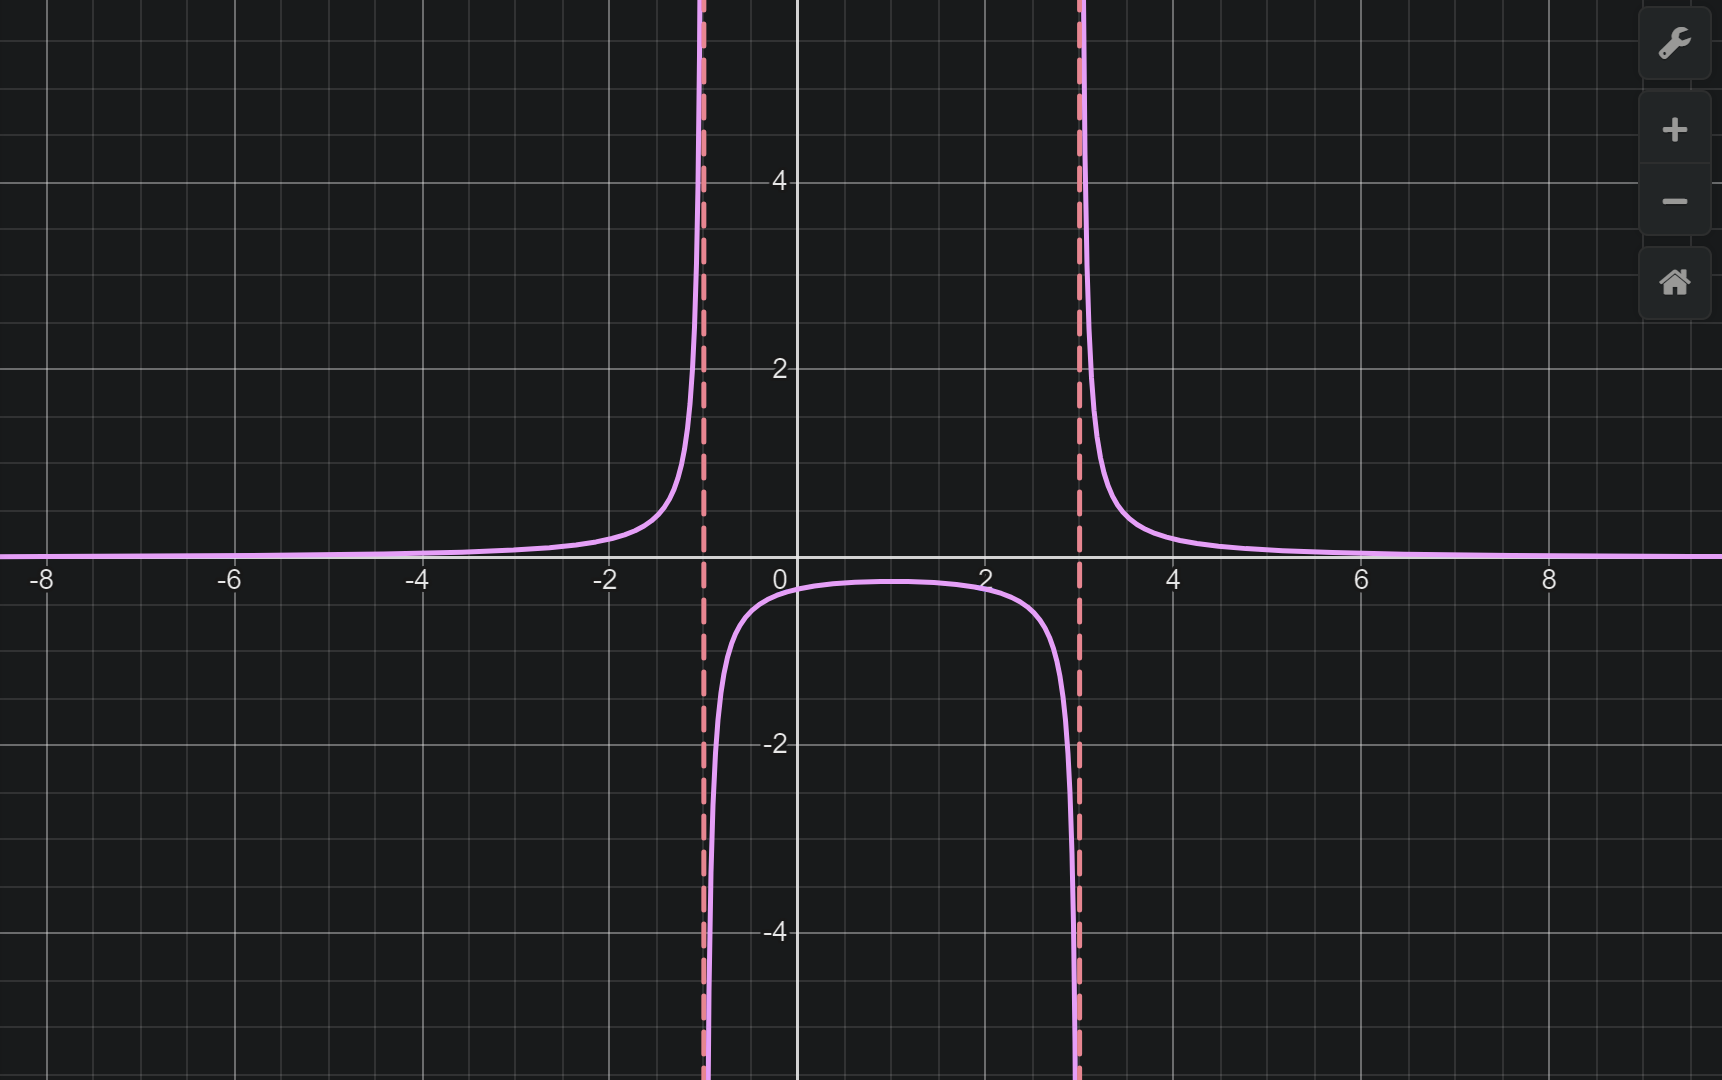
\includegraphics[width=0.9\textwidth]{imgs/graph(1_x+1_x-3).png}
    \end{figure}
\end{enumerate}
$x\to -1^-, y\to +\infty \quad x\to 3^-, y\to -\infty$ \quad $x\in(-\infty, -1)(3, +\infty) y >0$ \\
$x\to -1^+, y \to +\infty \quad x\to 3^+, y\to +\infty$ \quad $x\in(-1,3) y< 0$

\subsection{Reciprocals of Quadratic Functions}
A quadratic function has the form f (x) = ax2 + bx + c in
standard form, where a, b and c are real coefficients.\\
What does the graph of the reciprocal of a quadratic look
like?\\
There are three cases to consider, depending on the
factorability of the quadratic.
\subsubsection{Asymptotes}
Vertical asymptotes occur when the denominator of a
rational expression is zero. Thus, the roots of a quadratic expression in the denominator correspond to any vertical asymptotes.\\
Since a quadratic may have zero, one or two real roots, the
reciprocal of a quadratic may have zero, one or two vertical
asymptotes.\\

Like reciprocals of linear functions, horizontal asymptotes can
be determined by dividing each term by the highest power,
then evaluating as $x\to\infty$.
\subsection*{Example:}
Determine the equations of any asymptotes for
$$
f(x)=\frac{1}{x^2-4} \text {. }
$$

After factoring, $f(x)=\frac{1}{(x-2)(x+2)}$.
There are two vertical asymptotes: one with equation $x=-2$, and the other $x=2$.
Divide the expression by $x^2$ and let $x \rightarrow \infty$.
$$
\begin{aligned}
\frac{\frac{1}{x^2}}{\frac{x^2}{x^2}-\frac{4}{x^2}} & =\frac{0}{1-0} \\
& =0
\end{aligned}
$$
\subsection*{Asymptotes}

\begin{minipage}{0.6\textwidth}
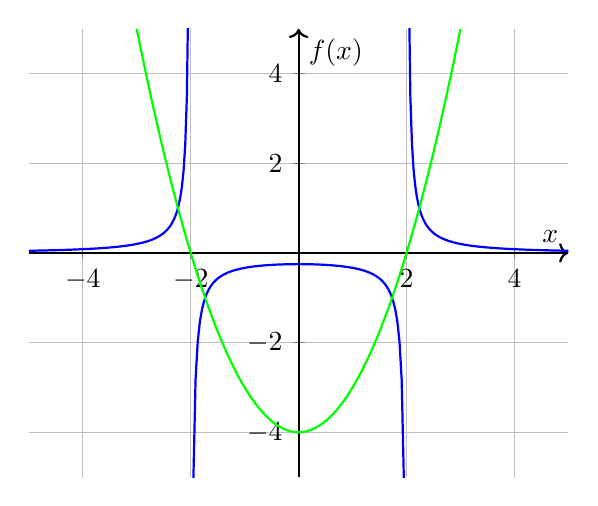
\begin{tikzpicture}
\begin{axis}[
    xlabel={$x$},
    ylabel={$f(x)$},
    xmin=-5, xmax=5,
    ymin=-5, ymax=5,
    axis lines=center,
    axis line style=->,
    legend pos=north west,
    samples=100,
    grid=major,
    thick
]
\addplot[blue,domain=-5:-2.01] {1/(x^2 - 4)};
\addplot[blue,domain=-1.99:1.99] {1/(x^2 - 4)};
\addplot[blue,domain=2.01:5] {1/(x^2 - 4)};
\addplot[green, domain=-3:3]{x^2-4};
\end{axis}
\end{tikzpicture}
\end{minipage}%
\begin{minipage}{0.4\textwidth}
$f(x)$ is symmetric about the same axis as $g(x)$. A local maximum occurs on $f(x)$ where there is a local minimum on $g(x)$.
\end{minipage}
\subsubsection{Intercepts}
As with any function, the f(x)-intercept can be found by
substituting $x = 0$ into its equation.\\
x-intercepts will occur when the numerator evaluates to zero.
If the reciprocal of a quadratic has the form
$$f(x) = \frac{1}{ax^2 + bx + c},$$ then there will always be a horizontal
asymptote at f (x) = 0.
Verifying the last example, the f (x)-intercept is at $\frac{1}{0^-4}=\frac{1}{4}$ and there are no x-intercepts.

\subsubsection{Minima/Maxima}
Since functions of the form $$f(x) = \frac{1}{ax^2 + bx + c},$$
have line symmetry, any minimum or maximum point will occur
halfway between the two vertical asymptotes.\\
Substituting in this middle value allows us to determine the
coordinate where there is a local min/max.
In the previous example, the vertical asymptotes were at $x = -2$ and $x = 2$.
Therefore, a local minimum or maximum will occur when\\
\begin{equation*}
    x=\frac{-2+2}{2}=0 \quad \text{or at} \quad \left(0, -\frac{1}{4}\right)
\end{equation*}
\subsection{Rational Functions of the Form $f(x)\frac{ax+b}{cx+d}$}
\textbf{Recall that a rational function is a ratio of two polynomial functions, $p(x)$ and $q(x)$, such that $f(x) = \frac{p(x)}{q(x)}$.} Since $q(x) \neq 0$, there will often be some form of discontinuity, such as an asymptote or a hole. In this section, we will investigate rational functions that have the form $f(x) = \frac{ax + b}{cx + d}$. Such functions have predictable properties, making them easy to graph.

\subsubsection*{Example}
\textbf{Graph the function $f(x) = \frac{x + 4}{x - 2}$ and describe its properties.} There is a vertical asymptote at $x = 2$. Dividing each term by $x$ to find the equation of the horizontal asymptote:
\[
\frac{x}{x} + \frac{4}{x} \div \frac{x}{x} - \frac{2}{x} = \frac{1 + 0}{1 - 0} = 1
\]
A horizontal asymptote occurs at $f(x) = 1$. The $x$-intercept is at $x = -4$ and the $f(x)$-intercept is at $-2$.

\begin{center}
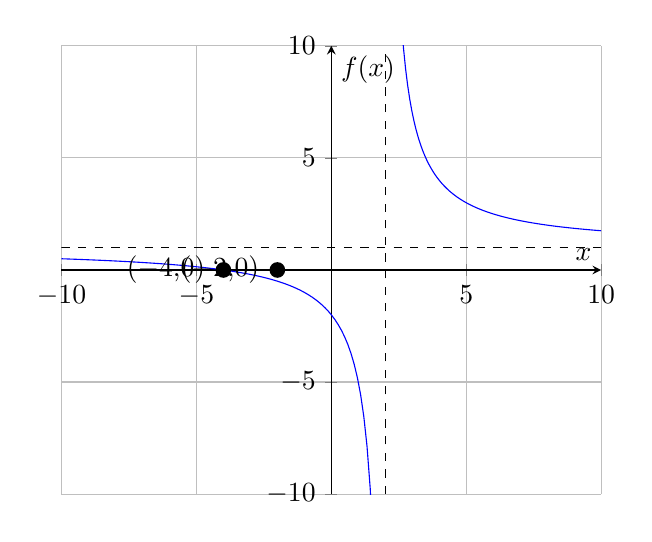
\begin{tikzpicture}
\begin{axis}[
    axis lines=middle,
    xlabel={$x$},
    ylabel={$f(x)$},
    xmin=-10, xmax=10,
    ymin=-10, ymax=10,
    xtick={-10,-5,...,10},
    ytick={-10,-5,...,10},
    grid=both,
    ]
    \addplot[domain=-10:1.8,blue,samples=100] {(x + 4)/(x - 2)};
    \addplot[domain=2.2:10,blue,samples=100] {(x + 4)/(x - 2)};
    \draw[dashed] (2,-10) -- (2,10);
    \draw[dashed] (-10,1) -- (10,1);
    \node[label={180:{($-4$,0)}},circle,fill,inner sep=2pt] at (-4,0) {};
    \node[label={180:{($-2$,0)}},circle,fill,inner sep=2pt] at (-2,0) {};
\end{axis}
\end{tikzpicture}
\end{center}

\subsubsection{Putting it Together}
To determine the function's behavior to the right of the vertical asymptote, test values of $x$ greater than $2$.

\subsubsection{Symmetry}
$f(4) = 4$ and $f(8) = 2$, resulting in a symmetric graph about the asymptotes.

\subsubsection{Complete Graph}
A complete graph of $f(x)$ confirms the symmetry.

\subsubsection*{Example 2}
\textbf{Graph the function $f(x) = \frac{2x - 1}{x + 1}$.} There is a vertical asymptote at $x = -1$. Dividing each term by $x$ to find the equation of the horizontal asymptote:
\[
\frac{2x}{x} - \frac{1}{x} \div \frac{x}{x} + \frac{1}{x} = \frac{2 - 0}{1 + 0} = 2
\]
A horizontal asymptote occurs at $f(x) = 2$. The $x$-intercept is at $\frac{1}{2}$ and the $f(x)$-intercept is at $-1$.

\begin{center}
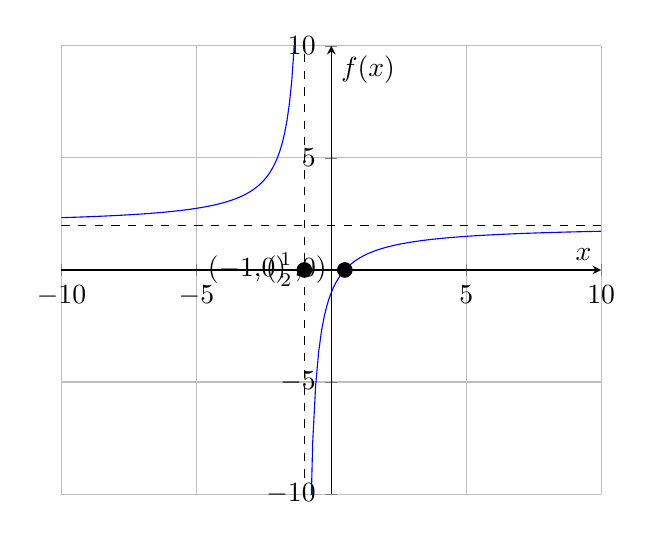
\begin{tikzpicture}
\begin{axis}[
    axis lines=middle,
    xlabel={$x$},
    ylabel={$f(x)$},
    xmin=-10, xmax=10,
    ymin=-10, ymax=10,
    xtick={-10,-5,...,10},
    ytick={-10,-5,...,10},
    grid=both,
    ]
    \addplot[domain=-10:-1.2,blue,samples=100] {(2*x - 1)/(x + 1)};
    \addplot[domain=-0.8:10,blue,samples=100] {(2*x - 1)/(x + 1)};
    \draw[dashed] (-1,-10) -- (-1,10);
    \draw[dashed] (-10,2) -- (10,2);
    \node[label={180:{($\frac{1}{2}$,0)}},circle,fill,inner sep=2pt] at (0.5,0) {};
    \node[label={180:{($-1$,0)}},circle,fill,inner sep=2pt] at (-1,0) {};
    
\end{axis}
\end{tikzpicture}
\end{center}

\subsubsection{Comparison}
Comparing the graphs of $f(x) = \frac{x+4}{x-2}$, $g(x) = \frac{x+3}{x-2}$, and $h(x) = \frac{x+2}{x-2}$.

\subsubsection{Properties}
All three functions have the form $\frac{ax + b}{cx + d}$. As the value of $b$ increases, the function is stretched further from the asymptotes. The value of $b$ has no effect on the vertical and horizontal asymptotes.

\subsubsection*{Example 3}
\textbf{Determine the equation of a rational function with the following features:}
\begin{itemize}
    \item A vertical asymptote at $x = 3$.
    \item A horizontal asymptote at $f(x) = 2$.
    \item An $x$-intercept at $x = 1$.
\end{itemize}
Since a vertical asymptote occurs at $x = 3$, let the denominator be $x - 3$. In order for a horizontal asymptote to occur at $f(x) = 2$, and since $c = 1$, the value of $a$ must be $2$, since $a/c = 2/1 = 2$. The $x$-intercept occurs when the numerator is zero, or $2x + b = 0$. Isolating $x$, this becomes $x = -\frac{b}{2}$. Since the $x$-intercept is $1$, $-\frac{b}{2} = 1$, or $b = -2$. Thus, a possible equation is $f(x) = \frac{2x - 2}{x - 3}$.


\subsection{Rational equations and inequalities}
To solve equations involving rational expressions, we have the freedom to clear out fractions before proceeding. After multiplying both sides by the common denominator, we are left with a polynomial equation.

\subsubsection*{Example:}
Solve the equation $\frac {2}{x} + \frac {3x}{x+1} = 4.$
\subsubsection*{Solution }
The common denominator is x(x+1). We multiply both sides by x(x+1)
 to clear out the fractions.
\begin{align*} 
      \frac{2}{x} + \frac{3x}{x+1} &= 4  \\
      x(x+1) \left( \frac{2}{x} + \frac{3x}{x+1} \right) &= x(x+1) ( 4 )\\
      x(x+1) \cdot \frac{2}{x}  + x(x+1) \cdot \frac{3x}{x+1} &= 4x(x+1)\\
      2(x+1) + 3x(x) &= 4x^2 + 4x\\
      3x^2 + 2x + 2 &= 4x^2 + 4x\\
      x^2 + 2x - 2 &= 0.
    \end{align*}
The quadratic formula gives solutions as $\displaystyle x = \dfrac {-2 \pm \sqrt {12}}{2} = -1 \pm \sqrt {3}$\\

If we look back at the original equation, we notice that there are some numbers that we are not allowed to plug in for \(x\). When \(x=0\) or \(x=-1\), the left-hand side of the equation is not defined due to a division by zero issue. Since neither \(-1 + \sqrt{3}\) nor \(-1 - \sqrt{3}\) have such an issue, they are both solutions.
\subsubsection{Inequalities}
When faced with nonlinear inequalities, such as those involving general rational functions, we make use of a sign chart. The inequality in the following example is not given in factored form, so we have some work to do.

\subsubsection*{Example}
Solve the inequality $\displaystyle x^2 + 5x \leq -10 -\dfrac {16}{x-2}$
\newpage
\subsubsection*{Solution}
We’ll begin by moving everything to one side, then combining them all together into a single fraction.

\begin{align*} 
         x^2 + 5x &\leq -10 -\dfrac{16}{x-2}\\
      x^2 + 5x +10 +\dfrac{16}{x-2} &\leq 0\\
      \left(x^2+5x+10\right) \cdot \left(\dfrac{x-2}{x-2}\right) +\dfrac{16}{x-2} &\leq 0\\
      \dfrac{x^3+3x^2-20}{x-2} + \dfrac{16}{x-2} &\leq 0\\    
      \dfrac{x^3+3x^2-4}{x-2} &\leq 0\\
      \dfrac{(x-1)(x+2)^2}{x-2} &\leq 0
    \end{align*}
    Now that the inequality is in a better form for us to work with, we’ll build a sign chart like we did in the last example.

    \begin{figure}[ht]
    \centering
    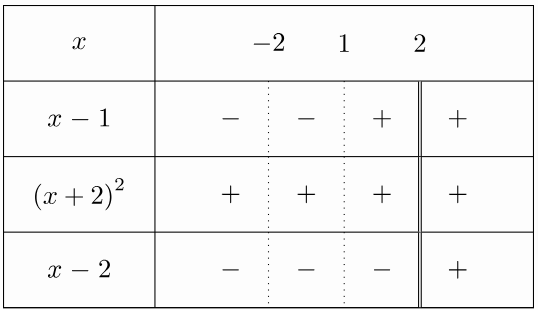
\includegraphics[width=0.9\textwidth]{imgs/graph figure.png}
    \end{figure}
We see from the chart that $\displaystyle \frac{(x-1)(x+2)^2}{x-2}$ will be negative in $(1,2)$. At $x=-2$ and $x=1$ it is zero. The solution is then: $(-2) \cup [1,2)$.
\newpage
\subsection{Making Connections With Rational Functions and Equation}
\textcolor{red}{Special cases} occur when a factored rational function has the exact same bracket in both the numerator and denominator. In this case, the
bracket would be crossed out on both the top and bottom and a statement reflecting a hole at that point would be made.
\newpage
\section*{Resources}
\begin{itemize}
    \item \href{https://ximera.osu.edu/calcwithreview/calculusWithReview/rationalFunctions/digInRationalEqIneq}{Rational equations and inequalities}
    \item \href{https://www.andrews.edu/~rwright/Precalculus-RLW/Text/02-07.html#:~:text=A%20vertical%20asymptote%20of%20a,inputs%20approach%20%E2%88%9E%20or%20%E2%80%93%E2%88%9E.}{Veritcal and horizontal asymptotes }
\end{itemize}

\end{document}